% =============================================
% =============================================
% Document class: Article
\documentclass[ a4paper, twoside, 11pt]{article}
% Packages: LaTeX (Depth-1)
\usepackage[ vlined, linesnumbered, ruled]{algorithm2e}
\usepackage{ amsfonts, amsmath, amssymb, amsthm}
\usepackage[ titletoc, title]{appendix}
\usepackage{ bbm}
\usepackage{ color}
\usepackage{ dsfont}
\usepackage{ enumitem}
\usepackage{ graphicx}
\usepackage{ fancyhdr, float, fullpage}
\usepackage{ hyperref}
\usepackage{ lastpage, latexsym, lipsum}
\usepackage{ mathrsfs, mathtools, multicol}
\usepackage{ parskip}
\usepackage{ setspace, stmaryrd, subcaption}
\usepackage{ tabularx}
\usepackage{ wasysym}
\usepackage[ dvipsnames, table]{ xcolor}
\usepackage{ xfrac}
% Packages: LaTeX (Depth-2)
\usepackage{ epstopdf}

% =============================================
\topmargin 			= -1.6cm
\headheight 		= .90cm
\headsep 			= .80cm
\textheight 		= 24.0cm
\textwidth 			= 15.5cm
\oddsidemargin		= 0.cm
\evensidemargin 	= 0.cm

% =============================================
% =============================================
% Macros: Language
\newcommand{\define}{\triangleq}
\newcommand{\done}{\hfill $\square$}
%\newcommand{\eqCIRC}{\stackrel{\circ}{=}}
%\newcommand{\eqSTAR}{\stackrel{*}{=}}
\renewcommand{\epsilon}{\varepsilon}
\newcommand{\eg}{\textit{e.g.,\;}}
\newcommand{\egc}{\textit{e.g.:\;}}
\newcommand{\Eg}{\textit{E.g.,\;}}
\newcommand{\Egc}{\textit{E.g.:\;}}
\newcommand{\ie}{\textit{i.e.,\;}}
\newcommand{\iec}{\textit{i.e.:\;}}
\newcommand{\Ie}{\textit{I.e.,\;}}
\newcommand{\Iec}{\textit{I.e.:\;}}
\newcommand{\QED}{\hfill $\blacksquare$}
\renewcommand{\tilde}[1]{\widetilde{#1}}
\newcommand{\tsup}[1]{\ensuremath{^{\text{#1}}}}
\newcommand{\tsub}[1]{\ensuremath{_{\text{#1}}}}
\renewcommand{\vec}[1]{{\boldsymbol{#1}}}

% Macros: Optimization & Probability
\DeclareMathOperator*{\argmax}{arg\,max}
\DeclareMathOperator*{\argmin}{arg\,min}
\newcommand{\Exp}{\mathbb{E}}
\newcommand{\Indicate}[1]{ \IndFun \, \{ \, #1 \, \} }
\renewcommand{\Pr}{\mathbb{P}}
\newcommand{\Normal}{\mathcal{N}}
\newcommand{\std}{\text{std}}
\newcommand{\var}{\text{var}}

% Macros: Sets
\newcommand{\Complex}{\mathbb{C}}
\renewcommand{\emptyset}{\varnothing}
\newcommand{\Nat}{\mathbb{N}}
\renewcommand{\Re}{\mathbb{R}}
\newcommand{\ReNN}{{\Re}_{\geq 0}}
\newcommand{\ReSP}{{\Re}_{> 0}}
\renewcommand{\subset}{\subseteq}
\renewcommand{\supset}{\supseteq}
\newcommand{\Z}{\mathbb{Z}}
\newcommand{\ZNN}{{\Z}_{\geq 0}}

% Macros: Spacing & Other Commands
\newcommand{\fullcut}{\vspace{-\baselineskip}}
\newcommand{\fullskip}{\vspace{\baselineskip}}
\newcommand{\halfcut}{\vspace{-0.5\baselineskip}}
\newcommand{\halfskip}{\vspace{0.5\baselineskip}}
\renewcommand{\figurename}{Figura}
\renewcommand{\tablename}{Tabla}

% =============================================
% Sesion de Clase
\newcommand{\sesion}{03}
% Macros para definiciones, teoremas, etc
\newcounter{sesion}
\setcounter{sesion}{\sesion}
\theoremstyle{definition}
\newtheorem{definition}{Definici\'on}[sesion]
\newtheorem{example}[definition]{Ejemplo}
\newtheorem{exercise}[definition]{Ejercicio}
\newtheorem{note}[definition]{Nota}
\newtheorem{problem}[definition]{Problema}
\newtheorem{theorem}[definition]{Teorema}

% =============================================
% =============================================
\newcommand{\HeaderLine}{}
\newcommand{\FooterLine}{P\'agina \thepage ~de \pageref*{LastPage}}

\pagestyle{fancyplain}
\fancyhf{}

\rhead[]{\fancyplain{}{\HeaderLine}}
\lhead[\fancyplain{}{\HeaderLine}]{}
\lfoot[\fancyplain{}{\FooterLine}]{}
\rfoot[]{\fancyplain{}{\FooterLine}}

\renewcommand{\headrulewidth}{0.4pt}
\renewcommand{\footrulewidth}{0.4pt}
\renewcommand{\thefootnote}{\fnsymbol{footnote}}

% =============================================
% =============================================
\begin{document}
\allowdisplaybreaks

\begin{center}
\Large Control Autom\'atico (FIMCP-03905): Examen \sesion \\[1ex]
\small \textbf{A\~no:} 2016-2017 \qquad \textbf{T\'ermino:} II \qquad
\textbf{Instructor:} Luis I. Reyes Castro \qquad \textbf{Paralelo:} 02
\end{center}
\halfskip

\fbox{

\begin{minipage}[b][\height][t]{\textwidth}
\vspace{0.2 cm}

\begin{center}
\textbf{COMPROMISO DE HONOR}
\end{center}
\vspace{0.4 cm}

\scriptsize
{
Yo, \rule{60mm}{.1pt} al firmar este compromiso, reconozco que el presente examen est\'a dise\~nado para ser resuelto de manera individual, que puedo usar un l\'apiz o pluma y una calculadora cient\'ifica, \linebreak que solo puedo comunicarme con la persona responsable de la recepci\'on del examen, y que cualquier instrumento de comunicaci\'on que hubiere tra\'ido debo apagarlo. Tambi\'en estoy conciente que no debo consultar libros, notas, \linebreak ni materiales did\'acticos adicionales a los que el instructor entregue durante el examen o autorice a utilizar. Finalmente, me comprometo a desarrollar y presentar mis respuestas de manera clara y ordenada. \\

Firmo al pie del presente compromiso como constancia de haberlo le\'ido y aceptado. 
\vspace{0.4 cm}

Firma: \rule{60mm}{.1pt} \qquad N\'umero de matr\'icula: \rule{42mm}{.1pt} \hspace{0.5cm} \\[-0.8ex]

}

\end{minipage}

}

\halfskip

\textbf{Instrucciones:} Cada uno de los siguientes cuatro problemas tiene un peso de 10 puntos. 
\halfskip

% =============================================
\begin{problem}
Construya un modelo de espacio de estados para el siguiente sistema mec\'anico rotacional, donde la entrada es el torque $T(t)$ y las salidas son las posiciones angulares de cada uno de los tres cuerpos. Por conveniencia, por favor denote el \'angulo del cuerpo del lado izquierdo como $\theta_0(t)$, el del cuerpo del lado derecho superior como $\theta_1(t)$, y el del cuerpo del lado derecho inferior como $\theta_2(t)$. 

\begin{figure}[htb]
\centering
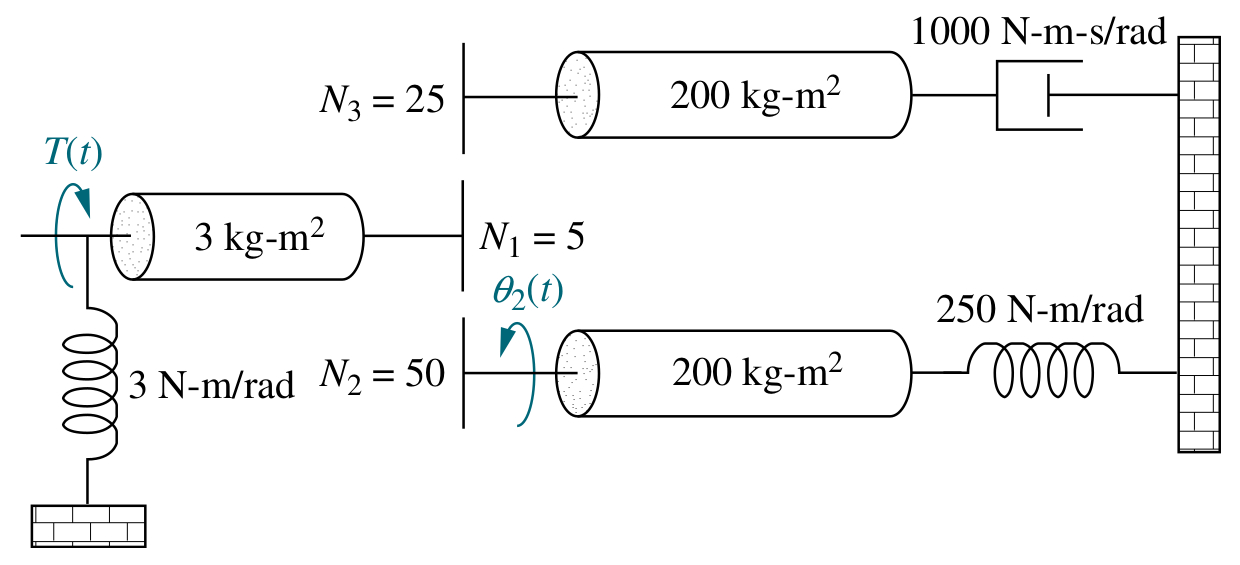
\includegraphics[ width = 0.62\textwidth]{fig_P2-20.jpg}
\end{figure}

\end{problem}
\vspace{\baselineskip}

% =============================================
\begin{problem}
Encuentre la funci\'on de transferencia de la entrada $\theta_{11}(s)$ a la salida $\theta_{22}(s)$ en el siguiente sistema, \ie la funci\'on de transferencia $G(s) = \theta_{22}(s) \, / \, \theta_{11}(s)$. 

\emph{Nota:} Suponga que la entrada $\theta_{12}(s)$ es nula. 

\begin{figure}[htb]
\centering
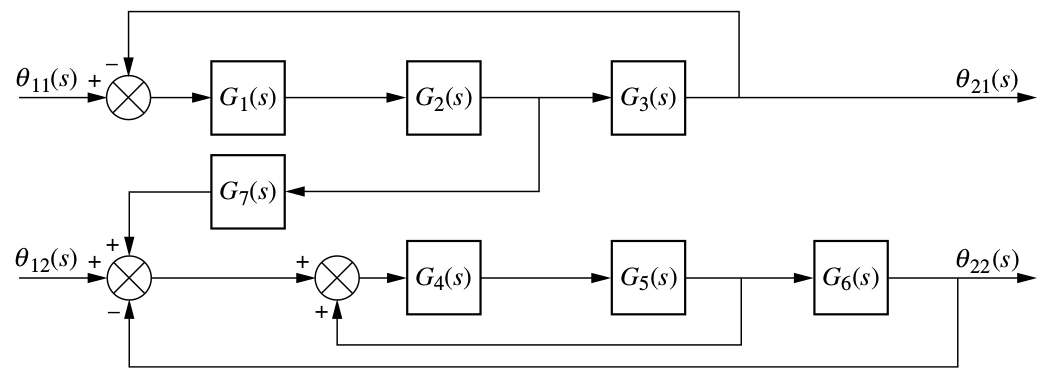
\includegraphics[ width = 0.88\textwidth]{fig_P5-8.jpg}
\end{figure}

\end{problem}
\vspace{\baselineskip}
\newpage

% =============================================
\begin{problem}
Considere un amplificador operacional en la configuraci\'on de divisor de voltage que estudiamos en clase, donde $Z_1(s)$ es la impidencia en la parte `superior' del circuito y $Z_2(s)$ es la impidencia en la parte `inferior'. En este caso la funci\'on de transferencia del amplificador es: 
\[
G(s) \, = \, \frac{Z_1(s) + Z_2(s)}{Z_2(s)}
\]
Con esto en mente: 
\begin{enumerate}[label=\alph*.]
\item Suponga que usted quiere construir un controlador PD con funci\'on de transferencia: 
\[
G_{PD}(s) \, = \, K_p + K_d \, s
\]
Indique como puede lograr esto si usted solo tiene dos capacitores $C_1$ y $C_2$ y una resistencia $R$. En particular, indique la arquitectura de su amplificador operacional, \linebreak su funci\'on de transferencia, y los valores de $C_1$, $C_2$ y $R$ como funci\'on de $K_p$ y $K_d$. 
\item Suponga que usted quiere construir un controlador PI con funci\'on de transferencia: 
\[
G_{PI}(s) \, = \, K_p + \frac{K_i}{s}
\]
Indique como puede lograr esto si usted solo tiene un capacitor $C$ y dos resistencias $R_1$ y $R_2$. En particular, indique la arquitectura de su amplificador operacional, \linebreak su funci\'on de transferencia, y los valores de $C$, $R_1$ y $R_2$ como funci\'on de $K_p$ y $K_i$. 

\end{enumerate}


\end{problem}
\vspace{\baselineskip}

% =============================================
\begin{problem}
Para el siguiente sistema: 
\begin{enumerate}[label=\alph*.]
\item Encuentre su funci\'on de transferencia como funci\'on de la ganancia $K$. 
\item Bosqueje su lugar geom\'etrico de las ra\'ices \emph{(root locus)}. Adem\'as, determine la veracidad o falsedad de cada uno de los siguientes enunciados: 
\begin{enumerate}[label=\roman*.]
\item El sistema es estable para todos los valores de la ganancia $K$. 
\item Existe un valor de la ganancia $K$ tal que si la ganancia excede ese valor entonces el sistema es inestable. 
\item Existe un valor de la ganancia $K$ tal que todos los polos son reales. 
\item Existe un valor de la ganancia $K$ tal que todos los polos son complejos conjugados. 
\end{enumerate}
\item Para $K = 20$ determine: 
\begin{enumerate}[label=\roman*.]
\item La estabilidad del sistema. 
\item Si el sistema es estable, determine la tasa de amortiguamiento y frecuencia natural de su(s) polo(s) dominante(s), junto con el error en estado estable del sistema. 
\end{enumerate}

\end{enumerate}

\begin{figure}[htb]
\centering
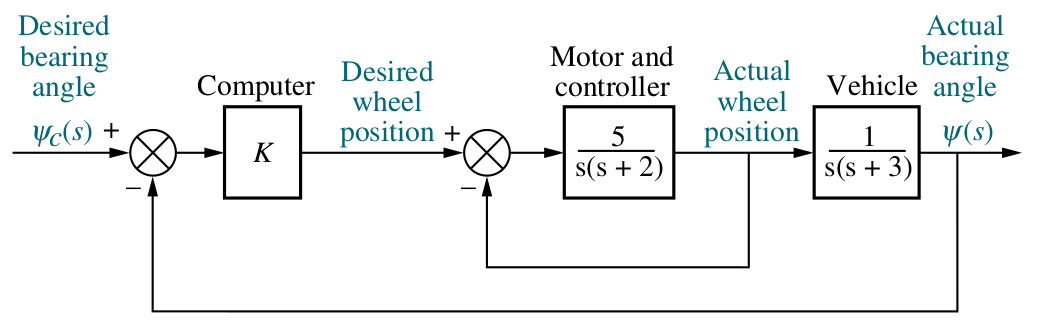
\includegraphics[ width = 0.76\textwidth]{fig_P5-35.jpg}
\end{figure}

\end{problem}
\vspace{\baselineskip}

\end{document}
